%% ============================================================
%%  Structured Transformer Pruning via Distillation-Guided
%%  Evolutionary Search with Adaptive Operator Selection
%%  NeurIPS 2025 style
%% ============================================================
\documentclass{article}

% ---------- NeurIPS style ----------
\usepackage[preprint]{neurips_2024}   % swap for [final] on submission

% ---------- encoding / fonts ----------
\usepackage[utf8]{inputenc}
\usepackage[T1]{fontenc}
\usepackage{microtype}

% ---------- math ----------
\usepackage{amsmath,amssymb,amsthm,mathtools}
\usepackage{bm}

% ---------- algorithms ----------
\usepackage{algorithm}
\usepackage{algorithmicx}
\usepackage{algpseudocode}
\algnewcommand\algorithmicforeach{\textbf{for each}}
\algdef{S}[FOR]{ForEach}[1]{\algorithmicforeach\ #1\ \algorithmicdo}

% ---------- graphics ----------
\usepackage{tikz}
\usetikzlibrary{
  arrows.meta, positioning, shapes.geometric,
  shapes.misc, fit, backgrounds, calc,
  decorations.pathreplacing, chains, matrix
}
\usepackage{pgfplots}
\pgfplotsset{compat=1.18}

% ---------- tables ----------
\usepackage{booktabs}
\usepackage{multirow}
\usepackage{array}

% ---------- misc ----------
\usepackage{graphicx}
\usepackage{subcaption}
\usepackage{hyperref}
\usepackage{cleveref}
\usepackage{xcolor}
\usepackage{enumitem}

% ---------- theorem environments ----------
\newtheorem{theorem}{Theorem}[section]
\newtheorem{proposition}[theorem]{Proposition}
\newtheorem{lemma}[theorem]{Lemma}
\newtheorem{corollary}[theorem]{Corollary}
\newtheorem{definition}[theorem]{Definition}
\newtheorem{remark}[theorem]{Remark}

% ---------- notation macros ----------
\newcommand{\Hb}{\mathbf{H}}
\newcommand{\nb}{\mathbf{n}}
\newcommand{\Sb}{\mathbf{S}}
\newcommand{\Vb}{\mathbf{V}}
\newcommand{\Zb}{\mathbf{Z}}
\newcommand{\Ab}{\mathbf{A}}
\newcommand{\Fb}{\mathbf{F}}
\newcommand{\wb}{\mathbf{w}}
\newcommand{\xb}{\mathbf{x}}
\newcommand{\yb}{\mathbf{y}}
\newcommand{\Cc}{\mathcal{C}}
\newcommand{\Fc}{\mathcal{F}}
\newcommand{\Ac}{\mathcal{A}}
\newcommand{\Mc}{\mathcal{M}}
\newcommand{\Pc}{\mathcal{P}}
\newcommand{\Sc}{\mathcal{S}}
\newcommand{\Lc}{\mathcal{L}}
\newcommand{\R}{\mathbb{R}}
\newcommand{\Zset}{\mathbb{Z}}
\newcommand{\E}{\mathbb{E}}
\newcommand{\bone}{\mathbf{1}}
\newcommand{\dcos}{d_{\mathrm{cos}}}
\newcommand{\dmag}{d_{\mathrm{mag}}}
\newcommand{\dblend}{d_{\alpha}}
\newcommand{\ddeep}{d_{\mathrm{deep}}}
\newcommand{\dstruct}{d_{\mathrm{struct}}}
\newcommand{\fsh}{f_{\mathrm{sh}}}
\newcommand{\MAC}{\mathrm{MAC}}
\newcommand{\clip}{\mathrm{clip}}
\newcommand{\argmax}{\mathop{\mathrm{arg\,max}}}
\newcommand{\argmin}{\mathop{\mathrm{arg\,min}}}
\newcommand{\argtop}{\mathop{\mathrm{arg\,top}}}

% ============================================================
\title{%
  Structured Transformer Pruning via\\
  Distillation-Guided Evolutionary Search\\
  with Adaptive Operator Selection
}

\author{Anonymous Authors}

\begin{document}
\maketitle

% ============================================================
\begin{abstract}
We present an evolutionary search algorithm for structured pruning
of transformer models that operates entirely within a hard MAC-budget
constraint.  Unlike methods that commit to a single-pass importance
ranking, our approach explores a combinatorial space of per-layer head
and neuron allocations through population-based search.
The core fitness signal is a multi-signal \emph{distillation distance}
that simultaneously penalises divergence in hidden-state residual
updates, attention branch activations, and feed-forward intermediate
representations at every layer, blending cosine and normalised
squared-error components with importance-weighted layer aggregation.
To navigate the exponentially large discrete search space efficiently
we contribute: (i)~an information-theoretic selection of orthogonal
training-free proxy metrics that guides a structure-aware
initialisation sweep; (ii)~an EXP3 bandit with implicit exploration
that adaptively allocates probability mass over a vocabulary of
sixteen mutation operators spanning both fine-grained budget-neutral
swaps and coarse architectural rewirings; (iii)~population-level
fitness sharing based on a blended structural distance to prevent
niche collapse; (iv)~MAP-Elites behavioural archiving and Pareto-front
tracking for multi-objective coverage of the accuracy-efficiency
trade-off; and (v)~a stagnation-aware adaptive scheduling mechanism
that continuously shifts the balance from local micro-mutations toward
structural macro-mutations and increases operator aggression as
improvement plateaus.  We prove that the repair operator produces
feasible candidates in finite steps and provide a regret bound for the
bandit component.  Experiments on BERT-base across GLUE benchmark tasks
demonstrate consistent improvements over gradient-based structured
pruning at matched compression ratios.
\end{abstract}

% ============================================================
\section{Introduction}
\label{sec:intro}

Pre-trained transformer language models have become the backbone of
modern natural-language processing, yet their deployment is bottlenecked
by quadratically scaling self-attention and large feed-forward
sublayers~\citep{vaswani2017attention}.  Structured pruning—removing
entire attention heads and FFN neurons rather than scattering individual
weights—directly reduces runtime, memory bandwidth, and accelerator
arithmetic without requiring sparse-tensor support~\citep{michel2019sixteen,voita2019analyzing}.

The central difficulty of structured pruning is \emph{co-adaptation}:
the optimal head count in one layer depends on how many neurons and
heads remain in every other layer.  One-shot importance-score methods
decide each component in isolation, ignoring this interdependence.
Architecture search approaches can in principle capture it, but the
discrete feasibility constraint (all allocations must stay within a
multiply-accumulate operation (MAC) budget) makes gradient-based
search non-trivial and renders most differentiable NAS methods
inapplicable without relaxation.

We frame the problem as constrained combinatorial optimisation and solve
it with a population-based evolutionary algorithm whose fitness function
is grounded in knowledge distillation.  The key idea is to measure each
candidate architecture by how faithfully it reproduces the teacher's
internal computation—not just its final output—using a multi-signal
distance that aggregates cosine and magnitude components across all
intermediate processing stages.

\paragraph{Contributions.}
\begin{enumerate}[leftmargin=*,label=(\roman*)]
  \item A formally grounded \textbf{multi-signal distillation distance}
        (\S\ref{sec:fitness}) that blends layer-residual, attention-branch,
        and FFN-branch signals under importance-weighted aggregation
        together with a capacity-cliff penalty.
  \item A \textbf{budget-feasible repair operator} (\S\ref{sec:repair})
        that protects the most important layers while trimming excess MAC
        cost; we prove it terminates in $O(LH + L P/\beta)$ steps.
  \item An \textbf{EXP3-IX bandit over a structured operator vocabulary}
        (\S\ref{sec:bandit}) with a niche-conditioned probability
        adjustment, together with an \textbf{adaptive stagnation
        schedule} that shifts operator mix and aggression online.
  \item A \textbf{proxy-guided structure-aware initialisation sweep}
        (\S\ref{sec:sweep}) that seeds the evolutionary population across
        the full range of affordable active-layer counts and head/neuron
        budget splits, providing strong warm starts.
  \item \textbf{Theoretical analysis}: a feasibility lemma for the repair
        operator and a regret bound for the bandit component.
\end{enumerate}

% ============================================================
\section{Related Work}
\label{sec:related}

\paragraph{Structured pruning.}
Early work prunes attention heads by magnitude or Taylor
importance~\citep{michel2019sixteen,voita2019analyzing,molchanov2019importance}.
Block-structured methods extend pruning to FFN neurons and whole
layers~\citep{xia2022structured,kwon2022fast}.  These approaches treat
each component independently and rely on a single-pass score; ours
searches the joint allocation space.

\paragraph{Architecture search for compression.}
Differentiable NAS~\citep{liu2019darts} requires relaxations that break
hard budget constraints.  Hardware-aware NAS~\citep{cai2019proxylessnas}
is closest in spirit but targets the design of new architectures rather
than pruning.  Recent zero-cost proxies~\citep{mellor2021neural,
chen2021neural} accelerate NAS but are used only for ranking, not as
evolutionary fitness.

\paragraph{Evolutionary methods.}
Evolutionary algorithms have been applied to network
pruning~\citep{liu2019metapruning,real2019regularized} and quantisation.
Our work differs in using a distillation-based fitness, an adaptive
multi-operator bandit, and structural fitness sharing designed
specifically for the joint head-neuron allocation space.

\paragraph{Knowledge distillation for pruning.}
Feature-level distillation~\citep{romero2014fitnets,
jiao2020tinybert,sun2020mobilebert} typically distills after
pruning.  We use the distillation distance as the \emph{search
objective}, evaluating every candidate against the intact teacher
without any fine-tuning.

% ============================================================
\section{Problem Formulation}
\label{sec:problem}

Consider a transformer with $L$ layers, each containing $H$ attention
heads and $P$ feed-forward neurons.  We parameterise a \emph{structured
pruning candidate} by
\begin{equation}
  \Cc = (\Hb,\, \nb),\quad
  \Hb \in \{0,1\}^{L\times H},\quad
  \nb \in \beta\Zset_{\ge 0}^{L},
  \label{eq:candidate}
\end{equation}
where $\Hb_{l,h}=1$ indicates that head $h$ of layer $l$ is active, and
$n_l$ is the number of active neurons in layer $l$, constrained to
integer multiples of a block size $\beta$ to align with hardware
efficiency.

\paragraph{MAC cost.}
Let $S$ denote the sequence length, $d$ the hidden dimension
($d_h = d/H$).  The per-head and per-neuron MAC costs are
\begin{equation}
  c_h = 4\,S\,d_h\,d, \qquad c_n = 2\,S\,d,
  \label{eq:mac_costs}
\end{equation}
and the total cost is
\begin{equation}
  \MAC(\Cc) = \sum_{l=1}^{L}
  \Bigl(\textstyle\sum_{h=1}^{H}\Hb_{l,h}\cdot c_h
        + n_l \cdot c_n\Bigr).
  \label{eq:mac}
\end{equation}

\paragraph{Active layers.}
Layer $l$ is \emph{active} iff $\sum_h \Hb_{l,h}>0$ and $n_l>0$.
Let $K(\Cc)$ denote the count of active layers.

\paragraph{Feasible set.}
Given MAC budget $\Omega$ and minimum active-layer count $K_{\min}$,
\begin{equation}
  \Fc = \bigl\{\Cc : \MAC(\Cc)\le\Omega,\; K(\Cc)\ge K_{\min}\bigr\}.
  \label{eq:feasible}
\end{equation}
The search minimises the distillation distance $d(\Cc)$
(defined in \S\ref{sec:fitness}) subject to $\Cc\in\Fc$.

% ============================================================
\section{Distillation-Based Fitness}
\label{sec:fitness}

\subsection{Multi-Signal Intermediate Distance}

We run the intact teacher model once per batch to collect reference
intermediate tensors.  The student is evaluated with head and neuron
masks applied via zero-gating.  At each layer $l$ we capture three
families of signals:
\begin{enumerate}[leftmargin=*,label=(\alph*)]
  \item \textbf{Hidden-state residual}: the additive contribution of
    layer $l$,
    $\bm{\Delta}^{(l)} = \Zb^{(l)} - \Zb^{(l-1)} \in \R^{B\times S\times d}$,
    where $\Zb^{(l)}$ is the full hidden state after layer $l$.
  \item \textbf{Attention branch}: the tensor $\Ab^{(l)}$ fed into the
    attention output projection (after head masking).
  \item \textbf{FFN branch}: the tensor $\Fb^{(l)}$ entering the
    feed-forward down-projection (after neuron masking).
\end{enumerate}

\paragraph{Blended per-signal distance.}
For matrices $\mathbf{X},\mathbf{Y}\in\R^{N\times d}$ of $N$ active tokens:
\begin{align}
  \dcos(\mathbf{X},\mathbf{Y})
    &= 1 - \frac{1}{N}\sum_{i=1}^{N}
       \frac{\xb_i^{\top}\yb_i}{\|\xb_i\|_2\|\yb_i\|_2},
  \label{eq:dcos} \\[4pt]
  \dmag(\mathbf{X},\mathbf{Y})
    &= \frac{\|\mathbf{X}-\mathbf{Y}\|_F^2}
           {\tfrac{1}{2}(\|\mathbf{X}\|_F^2+\|\mathbf{Y}\|_F^2)+\varepsilon},
  \label{eq:dmag}\\[4pt]
  \dblend(\mathbf{X},\mathbf{Y})
    &= (1-\alpha)\,\dcos(\mathbf{X},\mathbf{Y})
      + \alpha\,\dmag(\mathbf{X},\mathbf{Y}),
  \label{eq:dblend}
\end{align}
with $\alpha=0.35$.  The cosine component captures angular fidelity
while $\dmag$ penalises absolute magnitude collapse, which pure cosine
distance ignores.

\paragraph{Per-layer aggregation.}
Let $\Mc_l\subseteq\{\Delta,A,F\}$ be the set of signals available for
layer $l$.  The per-layer distance is
\begin{equation}
  d_l(\Cc)
  = \frac{1}{|\Mc_l|}
    \sum_{m\in\Mc_l}
    \dblend\!\bigl(\mathbf{S}^{(l,m)}_s,\,\mathbf{S}^{(l,m)}_t\bigr),
  \label{eq:dl}
\end{equation}
where the subscripts $s,t$ denote student and teacher tensors.

\paragraph{Importance-weighted depth distance.}
Let $w_l = \sum_h \Sb_{l,h}\,/\sum_{l',h}\Sb_{l',h}$ be the
normalised layer importance derived from head importance scores $\Sb$.
Define
\begin{equation}
  \ddeep(\Cc)
  = \sum_{l=1}^{L} \bar{w}_l\, d_l(\Cc),\qquad
  \bar{w}_l
  = \frac{w_l\cdot\bone[d_l\text{ available}]}
         {\sum_{j}w_j\cdot\bone[d_j\text{ available}]}.
  \label{eq:ddeep}
\end{equation}

\paragraph{Capacity-cliff penalty.}
Abrupt neuron-count drops across consecutive layers indicate a
processing bottleneck.  We penalise them with
\begin{equation}
  \Pc_{\mathrm{cliff}}(\Cc)
  = \kappa\sum_{l=1}^{L-1}\Bigl[\tfrac{n_l - n_{l+1}}{n_{\max}} - \delta\Bigr]_+
  + \rho\,\bone\!\Bigl[\tfrac{n_L}{n_{\max}} < \eta\Bigr],
  \label{eq:cliff}
\end{equation}
with $\kappa=2$, $\delta=0.25$, $\rho=0.5$, $\eta=0.10$.  The first
term discourages sharp drops along the depth axis; the second term
guards against an emaciated final layer.

\paragraph{Final fitness.}
\begin{equation}
  \boxed{
  d(\Cc)
  = \gamma\,\dcos\!\bigl(\Zb_s^{(L)},\Zb_t^{(L)}\bigr)
  + (1-\gamma)\,\ddeep(\Cc)
  + \Pc_{\mathrm{cliff}}(\Cc),
  \qquad \gamma = 0.35.}
  \label{eq:dfinal}
\end{equation}
The last-layer term $\dcos(\Zb_s^{(L)},\Zb_t^{(L)})$ provides a global
representation anchor; $\ddeep$ supplies fine-grained layer-by-layer
supervision; and $\Pc_{\mathrm{cliff}}$ enforces smooth neuron
utilisation.

\subsection{Evaluation Batches and Caching}

Teacher activations are pre-computed once over a fixed calibration set
drawn uniformly before the search.  All student evaluations are
performed under \texttt{torch.no\_grad()} using pre-packed batch
tensors.  Results are memoised by candidate signature (head mask bytes
$\oplus$ neuron-count bytes), so that repeated evaluations of
identical structures incur zero additional cost.

% ============================================================
\section{Algorithm}
\label{sec:algo}

Figure~\ref{fig:overview} summarises the five-phase pipeline.

% ------ TikZ: pipeline overview --------------------------------
\begin{figure}[t]
\centering
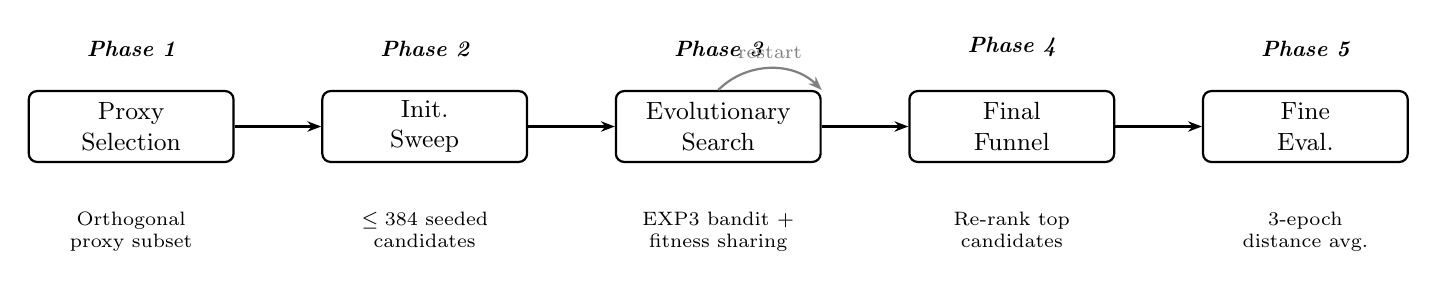
\begin{tikzpicture}[
  node distance = 7mm and 11mm,
  box/.style   = {draw, rounded corners=3pt, minimum width=2.6cm,
                  minimum height=0.9cm, font=\small, align=center,
                  thick},
  arr/.style   = {-{Stealth[length=5pt]}, thick},
  phase/.style = {draw, dashed, rounded corners=5pt,
                  inner sep=4pt, thick, gray}
]
% boxes
\node[box] (S1) {Proxy\\Selection};
\node[box, right=of S1] (S2) {Init.\\Sweep};
\node[box, right=of S2] (S3) {Evolutionary\\Search};
\node[box, right=of S3] (S4) {Final\\Funnel};
\node[box, right=of S4] (S5) {Fine\\Eval.};
% labels above
\node[above=3mm of S1, font=\footnotesize\itshape] {\textbf{Phase 1}};
\node[above=3mm of S2, font=\footnotesize\itshape] {\textbf{Phase 2}};
\node[above=3mm of S3, font=\footnotesize\itshape] {\textbf{Phase 3}};
\node[above=3mm of S4, font=\footnotesize\itshape] {\textbf{Phase 4}};
\node[above=3mm of S5, font=\footnotesize\itshape] {\textbf{Phase 5}};
% arrows
\draw[arr] (S1) -- (S2);
\draw[arr] (S2) -- (S3);
\draw[arr] (S3) -- (S4);
\draw[arr] (S4) -- (S5);
% annotations below
\node[below=5mm of S1, font=\scriptsize, align=center]
  {Orthogonal\\proxy subset};
\node[below=5mm of S2, font=\scriptsize, align=center]
  {$\le 384$ seeded\\candidates};
\node[below=5mm of S3, font=\scriptsize, align=center]
  {EXP3 bandit +\\fitness sharing};
\node[below=5mm of S4, font=\scriptsize, align=center]
  {Re-rank top\\candidates};
\node[below=5mm of S5, font=\scriptsize, align=center]
  {3-epoch\\distance avg.};
% feedback arc from S3 to S3 (warm restart)
\draw[arr, gray] (S3.north) [bend left=45]
  to node[above, font=\scriptsize, gray]{restart}(S3.north east);
\end{tikzpicture}
\caption{Five-phase pruning pipeline.  Phases 1--2 build a
  proxy-guided warm start.  Phase 3 is the main evolutionary loop
  (with warm restarts on stagnation).  Phases 4--5 perform final
  re-ranking.}
\label{fig:overview}
\end{figure}
% ---------------------------------------------------------------

\subsection{Training-Free Proxy Metrics}
\label{sec:proxies}

We define eleven scalar proxy metrics that estimate candidate quality
without any gradient computation.  Let $k_l = \sum_h \Hb_{l,h}$
denote active heads in layer $l$ and $a_{l,h}=\Hb_{l,h}S_{l,h}$ the
retained score.  All metrics are in Table~\ref{tab:proxies}.

\begin{table}[t]
\centering
\caption{Training-free proxy metrics.  $K=\sum_l k_l$ is total heads;
  $\mathcal{T}$ is the top-15\% set by importance score.}
\label{tab:proxies}
\small
\setlength{\tabcolsep}{4pt}
\begin{tabular}{@{}llp{6.5cm}@{}}
\toprule
Label & Formula & Intuition\\
\midrule
$\phi_1$ (SynFlow) &
  $\sum_l \log(\sum_h a_{l,h}+\varepsilon)$ &
  Log-product of retained importances; gradient-flow proxy.\\
$\phi_2$ (Harmonic cap.) &
  $K_a/\sum_{l:\mathrm{act.}} k_l^{-1}$ &
  Harmonic mean active heads; penalises layer bottlenecks.\\
$\phi_3$ (Critical ret.) &
  $|\mathcal{T}\cap\{\text{active}\}|/|\mathcal{T}|$ &
  Fraction of critical heads retained.\\
$\phi_4$ (Retention CV) &
  $-\mathrm{CV}(\{l_{\mathrm{ret},l}\}_{l:\mathrm{act.}})$ &
  Negative coefficient of variation of layer-wise retention ratios.\\
$\phi_5$ (Layer ratio) &
  $K_a/L$ &
  Fraction of active layers.\\
$\phi_6$ (Act. rank) &
  $\exp(-\sum_i p_i \ln p_i)$ &
  Entropy-based diversity of retained importances.\\
$\phi_7$ (Hessian trace) &
  $\sum_{l,h}\Hb_{l,h}S_{l,h}^{2}$ &
  Second-order importance proxy.\\
$\phi_8$ (Neuron flow) &
  $\sum_{l:\mathrm{act.}}\log n_l$ &
  Log-flow through neuron bottlenecks.\\
$\phi_9$ (H--N balance) &
  $-\frac{1}{K_a}\sum_{l:\mathrm{act.}}|k_l/H - n_l/P|$ &
  Head--neuron symmetry within each layer.\\
$\phi_{10}$ (Joint min) &
  $\min_{l:\mathrm{act.}}\min(k_l/H, n_l/P)$ &
  Minimum joint utilisation across active layers.\\
$\phi_{11}$ (Imp. ret.) &
  $\sum_{l,h}\Hb_{l,h}S_{l,h}/\sum_{l,h}S_{l,h}$ &
  Global fraction of total head importance retained.\\
\bottomrule
\end{tabular}
\end{table}

\subsubsection{Orthogonal Proxy Selection}

Given a sample of $N_s$ candidates, compute the proxy matrix
$\bm{\Phi}\in\R^{N_s\times 11}$ and select a subset
$\Sc\subseteq\{1,\ldots,11\}$ of at most $M$ proxies greedily:

\begin{enumerate}[leftmargin=*]
  \item Compute uniqueness $u_j = |\{\phi_j^{(1)},\ldots,\phi_j^{(N_s)}\}|/N_s$.
  \item Remove proxies with zero variance.
  \item Initialise $\Sc = \{\argmax_j u_j\}$.
  \item Repeat until $|\Sc|=M$: add
    $j^* = \argmax_{j\notin\Sc}\; u_j\bigl(1 - \max_{k\in\Sc}|\hat{r}_{jk}|\bigr)$,
    where $\hat{r}_{jk}$ is the sample Pearson correlation.
\end{enumerate}

The composite proxy score is
$\Phi(\Cc) = \sum_{j\in\Sc}\lambda_j\phi_j(\Cc)$ with
$\lambda_j \propto u_j$.

\subsection{Structure-Aware Initialisation Sweep}
\label{sec:sweep}

Before the main loop we generate up to $N_{\mathrm{sweep}}=384$
diverse seed candidates by exhaustively varying four axes:

\begin{itemize}[leftmargin=*]
  \item \textbf{Active-layer count} $K \in [K_{\min}, K_{\max}]$
        (every affordable value).
  \item \textbf{Layer selection mode}: top-$K$ by importance,
        importance-weighted sampling, noisy top-$K$, top-bottom mix,
        middle-band, staggered stride, and uniform random.
  \item \textbf{Budget shape}: uniform, top-heavy (linearly increasing),
        bottom-heavy, and midpoint-peak (sinusoidal profile).
  \item \textbf{Head-fraction} $\rho_h \in \{0.25, 0.40, 0.55, 0.70\}$
        (fraction of MAC budget allocated to heads).
\end{itemize}

Per active-layer-count quota $q = 24$ ensures all affordable depths are
equally represented.  Each seed is scored with $\Phi(\Cc)$ and the
highest-scoring candidate initialises the search population.

\subsection{Budget Repair Operator}
\label{sec:repair}

\begin{algorithm}[t]
\caption{Budget Repair $\mathcal{R}(\Cc; \Omega, K_{\min}, H_{\min}, H_{\max})$}
\label{alg:repair}
\begin{algorithmic}[1]
\Require candidate $\Cc=(\Hb,\nb)$, budget $\Omega$, floors $K_{\min}, H_{\min}$
\State $\Lc_{\mathrm{prot}} \gets \argtop_{K_{\min}} \{w_l\}_{l=1}^L$
\Comment{protect most important layers}
\For{$l \in \Lc_{\mathrm{prot}}$}
  \If{$\sum_h\Hb_{l,h}<1$} add highest-scored inactive head in layer $l$ \EndIf
  \If{$n_l < \beta$} $n_l \gets \beta$ \EndIf
\EndFor
\State Enforce $H_{\min} \le \sum_{l,h}\Hb_{l,h} \le H_{\max}$ by greedy add/remove
\While{$\MAC(\Cc) > \Omega$}
  \State $\text{can\_prune\_n} \gets \exists l: n_l \ge 2\beta$
  \State $\text{can\_prune\_h} \gets \exists l: \sum_h\Hb_{l,h}>1$
  \If{$\text{can\_prune\_n}$ \textbf{and} $\mathrm{Uniform}(0,1)<0.6$}
    \State Remove one $\beta$-block from $\argmax_l n_l$
  \ElsIf{$\text{can\_prune\_h}$}
    \State Remove lowest-scored active head from $\argmax_l \sum_h\Hb_{l,h}$
  \Else
    \State Deactivate least-important unprotected active layer
  \EndIf
\EndWhile
\State \Return $\Cc$
\end{algorithmic}
\end{algorithm}

\begin{lemma}[Budget Feasibility]
\label{lem:repair}
Suppose $\Omega \ge K_{\min}(c_h + \beta c_n)$.  Then
Algorithm~\ref{alg:repair} terminates in at most
$LH + \sum_l n_l/\beta$ iterations and produces
$\mathcal{R}(\Cc)\in\Fc$.
\end{lemma}
\begin{proof}
Each iteration of the while loop reduces $\MAC(\Cc)$ by at least
$\delta_{\min}:=\min(c_h,\, \beta c_n)>0$ (either one head costs $c_h$
or one block costs $\beta c_n$).  The loop terminates no later than
after $\lceil(\MAC(\Cc)-\Omega)/\delta_{\min}\rceil$ iterations, which
is bounded by $LH+\sum_l n_l/\beta$ from above since each step removes
at most one head or one neuron block.

The invariant $K(\Cc)\ge K_{\min}$ is preserved because the ``else''
branch (deactivating an unprotected layer) is only reached when
protected layers alone cannot be trimmed further.  At that point,
the protected core has cost $K_{\min}(c_h+\beta c_n)\le\Omega$
by assumption, so the loop condition $\MAC(\Cc)>\Omega$ is violated
before all active layers are removed, and the branch is never executed
more times than there are unprotected active layers.
\end{proof}

\subsection{Bandit-Guided Operator Selection}
\label{sec:bandit}

\subsubsection{Operator Vocabulary}

Sixteen mutation operators divide into two classes:

\paragraph{Micro operators} (budget-neutral, fine-grained):
\emph{head swap} (move the weakest active head from a low-importance
layer to the best slot in a high-importance layer);
\emph{neuron swap} (transfer $\beta$ neurons between layers);
\emph{head-for-neurons} (trade one head for proportionally many neuron
blocks);
\emph{neurons-for-head} (reverse);
\emph{Lamarckian greedy} (locally optimise each layer's head
selection);
\emph{sparsity shift} (random neuron-block transfer);
\emph{neuron rebalance} (redistribute blocks proportionally to head
counts);
\emph{equilibrium mutate} (reduce the denser dimension in layers where
head/neuron fractions diverge);
\emph{jitter} (stochastic removal of heads/blocks with low probability).

\paragraph{Macro operators} (structural):
\emph{layer drop} (zero-out the least important active layer);
\emph{layer activate} (revive the most important dormant layer);
\emph{multi-drop} (apply layer drop 2--4 times);
\emph{head-neuron trade} (iterative exchange of head and neuron budget
across layers);
\emph{macro budget shift} (bulk transfer between randomly chosen donor
and receiver groups);
\emph{group reallocate} (concentrate budget in top-ranked layers,
drawing from lower-ranked ones);
\emph{layer rewire} (deactivate the $k$ weakest active layers, revive
$k$ dormant layers with the transferred head/neuron budgets).

\paragraph{Crossover.}
Three modes, sampled with probabilities $[0.45, 0.30, 0.25]$:
\begin{enumerate}[leftmargin=*,label=(\roman*)]
  \item \emph{Topology-budget}: adopt the layer-activation pattern from
    one parent, head/neuron budgets from the other (aligned by
    importance rank).
  \item \emph{Group swap}: layers $[0,c)$ from parent 1, layers
    $[c,L)$ from parent 2, at a random cut point $c$.
  \item \emph{Layerwise}: for each layer independently, inherit from
    parent~1 or~2 with equal probability.
\end{enumerate}

\subsubsection{EXP3-IX Update Rule}

We maintain a weight vector $\wb(t)\in\R_{>0}^K$ over the $K=16$
operators.  At each call the sampling distribution is
\begin{equation}
  p_k(t)
  = (1-\gamma)\frac{w_k(t)}{\sum_j w_j(t)} + \frac{\gamma}{K},
  \label{eq:exp3_probs}
\end{equation}
with exploration rate $\gamma=0.07$.  After executing operator $k$ and
observing reward $r\in[0,1]$, the \emph{implicit-exploration}
correction~\citep{neu2015explore} gives the unbiased importance-weighted
estimator
\begin{equation}
  \hat{r}_k(t) = \frac{r}{p_k(t) + \gamma},
  \label{eq:ix_est}
\end{equation}
and the multiplicative weight update is
\begin{equation}
  w_k(t+1)
  = w_k(t)\exp\!\Bigl(\frac{\gamma\,\hat{r}_k(t)}{K}\Bigr).
  \label{eq:exp3_update}
\end{equation}
Weights are periodically renormalised when $\max_k w_k(t)>10^6$ to
prevent overflow.

\paragraph{Reward construction.}
Let $d^*$ be the global best distance, $d_p$ the parent's distance, and
$\sigma_d = \max_i d_i - \min_i d_i + \varepsilon$ the empirical
distance range over recently evaluated candidates.  The reward is
\begin{equation}
  r(t) = 0.85\, r_{\mathrm{local}}(t) + 0.15\, r_{\mathrm{global}}(t),
  \label{eq:reward}
\end{equation}
\begin{equation}
  r_{\mathrm{local}}(t)
  = \tfrac{1}{2} + \tfrac{1}{2}\,
  \clip\!\Bigl(\tfrac{d_p - d_c}{2\sigma_d},\,-1,\,1\Bigr),
  \label{eq:reward_local}
\end{equation}
\begin{equation}
  r_{\mathrm{global}}(t)
  = \begin{cases}
      1.0 & d_c < d^*_{\mathrm{global}}, \\
      0.7 & d_c < d^*_{\mathrm{local}}, \\
      0.3 & \text{otherwise,}
    \end{cases}
  \label{eq:reward_global}
\end{equation}
where $d_c$ is the child's distance and $d^*_{\mathrm{local}}$ is the
current population's best.

\paragraph{Regret.}  The implicit-exploration estimator~\eqref{eq:ix_est}
satisfies $\hat r_k\le 1/(p_k+\gamma)$, bounding variance.  By the
standard EXP3-IX analysis~\citep{neu2015explore} the expected cumulative
regret after $T$ rounds is
\begin{equation}
  R_T \le 2\sqrt{KT\ln K},
  \label{eq:regret}
\end{equation}
independent of reward variance, i.e.\ the algorithm's cumulative reward
is within $O(\sqrt{KT\ln K})$ of the best fixed operator in hindsight.
(Proof deferred to Appendix~\ref{app:regret}.)

\subsubsection{Niche-Conditioned Operator Probabilities}

To exploit structural patterns in the search space, each candidate is
assigned a \emph{niche descriptor}
\begin{equation}
  \psi(\Cc) = \bigl(K(\Cc),\; \mathrm{mac\_bucket}(\Cc),\;
               \mathrm{shape\_bucket}(\Cc)\bigr),
\end{equation}
where mac\_bucket $\in \{\text{low},\text{mid},\text{high}\}$ and
shape\_bucket $\in \{\text{head\_heavy},\text{balanced},
\text{neuron\_heavy}\}$ are determined by MAC utilisation and the
head/neuron fraction balance respectively.  Per-niche operator success
rates $q_{k,\psi}\in[0,1]$ are updated online.  The effective sampling
probability blends the global bandit probabilities with niche-specific
estimates:
\begin{equation}
  \tilde{p}_k(\psi,t)
  \propto p_k(t)\cdot\bigl(0.5 + q_{k,\psi}(t)\bigr).
  \label{eq:niche_blend}
\end{equation}

\subsection{Fitness Sharing and Diversity}
\label{sec:sharing}

\paragraph{Structural distance.}
\begin{equation}
  \dstruct(\Cc_1,\Cc_2)
  = \frac{|\Hb_1\oplus\Hb_2|_0}{2LH}
  + \frac{\sum_l|n_{1,l}-n_{2,l}|}{2L(\max_{l}\max(n_{1,l},n_{2,l})+1)},
  \label{eq:dstruct}
\end{equation}
where $\oplus$ denotes elementwise XOR and the two halves give equal
weight to head-mask edit distance and neuron-count deviation.

\paragraph{Sharing and niche count.}
\begin{align}
  \mathrm{sh}(\Cc_i,\Cc_j)
    &= \max\!\Bigl(0,\, 1-\tfrac{\dstruct(\Cc_i,\Cc_j)}{\sigma_{\mathrm{sh}}}\Bigr),
  \label{eq:sh}\\
  \mu_i &= 1 + \textstyle\sum_{j\neq i}\mathrm{sh}(\Cc_i,\Cc_j).
  \label{eq:niche_count}
\end{align}

\paragraph{Adjusted fitness.}
\begin{equation}
  \fsh(\Cc_i)
  = \begin{cases}
      f(\Cc_i)/\mu_i & f(\Cc_i)\ge 0,\\
      f(\Cc_i)\cdot\mu_i & f(\Cc_i)<0,
    \end{cases}
  \label{eq:fsh}
\end{equation}
where $f(\Cc_i) = -d_c(\Cc_i)$ is the (sign-flipped) cheap
two-stage distance (\S\ref{sec:twoeval}).

\begin{proposition}[Isolation preserves fitness]
\label{prop:isolation}
If $\dstruct(\Cc_i,\Cc_j)\ge\sigma_{\mathrm{sh}}$ for all $j\neq i$,
then $\fsh(\Cc_i)=f(\Cc_i)$.
\end{proposition}
\begin{proof}
Each sharing term $\mathrm{sh}(\Cc_i,\Cc_j)=0$, giving $\mu_i=1$.
\end{proof}

\begin{proposition}[Crowding penalty]
\label{prop:crowding}
For any fixed raw fitnesses, $\fsh(\Cc_i)$ is strictly decreasing in
$|\mathcal{N}_i|:=|\{j:\dstruct(\Cc_i,\Cc_j)<\sigma_{\mathrm{sh}}\}|$
when all pairwise distances in $\mathcal{N}_i$ are equal.  Hence
selection pressure opposes structural crowding.
\end{proposition}
\begin{proof}
Under the equidistance assumption, $\mu_i=1+|\mathcal{N}_i|/c$ for
some constant $c>0$.  For $f>0$: $\partial\fsh/\partial|\mathcal{N}_i|
= -f/(c\mu_i^2)<0$.
\end{proof}

The niche-count matrix is computed in a single vectorised pass using
the structural distance matrix $\bm{D}\in\R^{N\times N}$,
enabling $O(N^2 LH)$ total complexity for a population of size $N$.

\subsection{Two-Stage Candidate Screening}
\label{sec:twoeval}

Evaluating all offspring at full token length is prohibitively
expensive.  We use a two-stage protocol:

\begin{enumerate}[leftmargin=*]
  \item \textbf{Cheap screening}: evaluate every offspring against
    $T_c=2048$ tokens to obtain a coarse distance $d_c(\Cc)$.
  \item \textbf{Full evaluation}: a diversity-aware subset of at most
    $K_{\mathrm{full}}=36$ candidates is selected and evaluated at
    $T_f=12288$ tokens.
\end{enumerate}

Selection for full evaluation proceeds greedily.  Let $\mathcal{Q}$
denote a per-active-layer-count quota of $q=2$.  We first fill each
active-layer-count quota by cheapest-first order, then augment with

\begin{equation}
  \mathrm{score}_{\mathrm{full}}(i)
  = -d_c(\Cc_i)
  + 0.30\min_{j\in\Sc_{\mathrm{full}}}\dstruct(\Cc_i,\Cc_j)
  + 0.10\,\mathrm{ActiveBonus}(i),
  \label{eq:sel_full}
\end{equation}
where $\mathrm{ActiveBonus}(i)=(1+|\{j:K(\Cc_j)=K(\Cc_i)\}|)^{-1}$
rewards underrepresented active-layer counts.  Only full evaluations
drive bandit updates and archiving.

\subsection{MAP-Elites Archiving}
\label{sec:mapelites}

A MAP-Elites archive~\citep{mouret2015illuminating} partitions candidates
by a two-dimensional behaviour descriptor
\begin{equation}
  \psi_{\mathrm{ME}}(\Cc)
  = \Bigl(K(\Cc),\;
    \bigl\lfloor 10\cdot\rho_h(\Cc)\bigr\rfloor\cdot 0.1\Bigr),
\end{equation}
where $\rho_h(\Cc) = \MAC_h(\Cc)/\MAC(\Cc)$ is the fraction of MAC
cost attributed to heads.  Each cell retains the candidate with minimum
distance; the archive stores at most one candidate per
$(K_{\mathrm{active}}, \hat{\rho}_h)$ cell.  This promotes coverage of
both depth-diversity and head/neuron-ratio diversity simultaneously.

\paragraph{Pareto archive.}  We additionally maintain a non-dominated
archive on the bi-objective space (distance, MACs), with crowded-distance
pruning to a capacity of 100 points.  This archive drives the final
funnel re-ranking and provides a visual trade-off curve.

\subsection{Adaptive Stagnation Scheduling}
\label{sec:schedule}

The macro-operator fraction and operator aggression are scheduled as
functions of the current stagnation counter $\tau$ (generations since
last improvement):

\begin{equation}
  \rho_{\mathrm{macro}}(\tau)
  = \min\bigl(0.80,\; 0.35 + 0.03\,\tau\bigr),
  \label{eq:macro_frac}
\end{equation}
\begin{equation}
  \xi(\tau) = 1 + 0.025\,\tau.
  \label{eq:aggression}
\end{equation}

At $\tau=0$ the population is dominated by fine-grained micro-mutations
($65\%$); as stagnation accumulates the balance shifts continuously
toward structural macro-mutations, reaching $80\%$ macro at
$\tau\approx 15$.  Simultaneously, operator aggression $\xi$ scales
the number and magnitude of transformations applied per call.

\paragraph{Warm restart.}
When $\tau=\tau_{\mathrm{stag}}=20$, the population is re-seeded.  Seeds
are drawn temperature-weighted from the best-ever candidate archive
$\Mc$ (capacity $C_{\mathrm{hof}}=50$):
\begin{equation}
  P(\Cc^*_i \text{ drawn})\propto\exp(-d_i/T_{\mathrm{hof}}),
  \quad T_{\mathrm{hof}}=0.5.
  \label{eq:hof_sample}
\end{equation}
Each seed $\Cc^*$ generates $p=4$ perturbation-level variants
$\Cc^{*(k)} = \mathcal{R}(\mathrm{op}^{2k}(\Cc^*))$ for
$k=1,\ldots,p$, where op is a randomly chosen budget-neutral operator
applied $2k$ times.  The cosine annealing temperature is simultaneously
reset to its initial value.

\subsection{Selection and Main Loop}

Algorithm~\ref{alg:main} summarises the generation loop.

\begin{algorithm}[t]
\caption{Main Evolutionary Search Loop (one generation)}
\label{alg:main}
\begin{algorithmic}[1]
\Require population $\mathcal{P}_t$, bandit $\wb(t)$, archives
         $\Mc,\Ac_{\mathrm{ME}},\Ac_{\mathrm{Pareto}}$,
         stagnation $\tau$
\State Evaluate $d_c(\Cc)$ for every $\Cc\in\mathcal{P}_t$
\State Compute structural distance matrix $\bm{D}$
\State Compute shared fitness $\{\fsh(\Cc)\}$ via Eq.~\eqref{eq:fsh}
\State $\rho_M \gets \rho_{\mathrm{macro}}(\tau)$;\quad
       $\xi \gets \xi(\tau)$
\State Select $N/2$ parents via tournament with novelty bonus
\State \textbf{Generate offspring:}
\For{$i = 1$ \textbf{to} $N$}
  \State $\text{mode} \gets$ \textsc{micro} if $i \le N(1-\rho_M)$,
         else \textsc{macro}
  \If{$\mathrm{Uniform}(0,1)<\rho_{\mathrm{xover}}(\text{mode})$}
    \State child $\gets$ crossover(parent$_1$, parent$_2$)
  \Else\; child $\gets$ clone(parent)
  \EndIf
  \State $k \gets$ sample from $\tilde{p}_k(\psi(\text{parent}), t)$
         via Eq.~\eqref{eq:niche_blend}
  \State child $\gets$ operator$_k$(child, $\xi$);\quad
         child $\gets \mathcal{R}(\text{child})$
\EndFor
\State Deduplicate offspring by structural $\sigma$-covering (greedy)
\State Select $K_{\mathrm{full}}\le 36$ for full evaluation via Eq.~\eqref{eq:sel_full}
\For{each fully-evaluated child $\Cc_c$ with distance $d_c$}
  \State Update bandit via Eqs.~\eqref{eq:ix_est}--\eqref{eq:exp3_update}
  \State Update $\Mc$, $\Ac_{\mathrm{ME}}$, $\Ac_{\mathrm{Pareto}}$
\EndFor
\State $\mathcal{P}_{t+1} \gets$ greedy $\sigma$-diverse merge of
       elites $\cup$ offspring $\cup$ $\mathcal{P}_t$
\If{no improvement} $\tau \gets \tau+1$;
  if $\tau=\tau_{\mathrm{stag}}$ then warm restart \EndIf
\end{algorithmic}
\end{algorithm}

\begin{figure}[t]
\centering
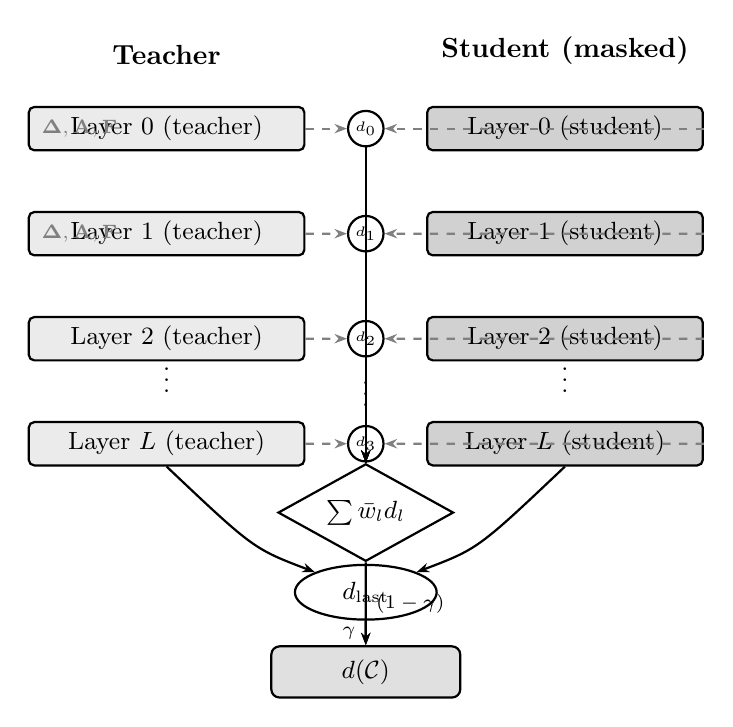
\begin{tikzpicture}[
  scale=0.92,
  font=\small,
  layer/.style={draw, rectangle, minimum width=3.5cm,
                minimum height=0.55cm, rounded corners=2pt, thick},
  sig/.style={draw, circle, minimum size=0.45cm, thick, inner sep=1pt,
              font=\tiny},
  arr/.style={-{Stealth[length=4.5pt]}, thick},
  darr/.style={-{Stealth[length=4.5pt]}, thick, dashed, gray}
]

% Teacher column
\foreach \l/\lab in {0/0,1/1,2/2,3/$L$}{
  \node[layer, fill=black!8] (T\l) at (0, -\l*1.45)
    {\small Layer \lab\ (teacher)};
}
\node[above=4mm of T0, font=\normalsize\bfseries] {Teacher};

% Student column
\foreach \l/\lab in {0/0,1/1,2/2,3/$L$}{
  \node[layer, fill=black!18] (S\l) at (5.5, -\l*1.45)
    {\small Layer \lab\ (student)};
}
\node[above=4mm of S0, font=\normalsize\bfseries] {Student (masked)};

% Distance nodes
\foreach \l in {0,1,2,3}{
  \node[sig] (D\l) at (2.75, -\l*1.45) {$d_{\l}$};
  \draw[darr] (T\l.east) -- (D\l);
  \draw[darr] (S\l.east) -- (D\l);
}

% Aggregation
\node[draw, diamond, aspect=1.8, thick, minimum width=1.9cm,
      minimum height=0.7cm, font=\small] (AGG) at (2.75, -5.3)
  {$\sum \bar{w}_l d_l$};
\foreach \l in {0,1,2,3}{
  \draw[arr] (D\l.south) -- (AGG.north);
}

% Last layer
\node[draw, ellipse, thick, minimum width=1.8cm, minimum height=0.65cm,
      font=\small] (LAST) at (2.75, -6.4) {$d_{\mathrm{last}}$};
\draw[arr] (T3.south) .. controls (1.2,-5.8) .. (LAST.north west);
\draw[arr] (S3.south) .. controls (4.3,-5.8) .. (LAST.north east);

% Final distance
\node[draw, rounded corners=3pt, thick, minimum width=2.4cm,
      minimum height=0.65cm, font=\small, fill=black!12] (FIN) at (2.75,-7.5)
  {$d(\Cc)$};
\draw[arr] (AGG) -- (FIN) node[midway,right,font=\scriptsize] {$(1-\gamma)$};
\draw[arr] (LAST) -- (FIN) node[midway,left,font=\scriptsize] {$\gamma$};

% Signal labels
\node[font=\scriptsize, gray] at (-1.2, -0.0) {$\bm\Delta,\mathbf{A},\mathbf{F}$};
\node[font=\scriptsize, gray] at (-1.2, -1.45) {$\bm\Delta,\mathbf{A},\mathbf{F}$};

% Dots
\node at (0, -2.45*1.45+0.2) {\vdots};
\node at (5.5, -2.45*1.45+0.2) {\vdots};
\node at (2.75, -2.45*1.45) {\vdots};

\end{tikzpicture}
\caption{Distillation distance computation.  At each layer three signal
  families ($\bm{\Delta}$: residual update; $\mathbf{A}$: attention
  branch; $\mathbf{F}$: FFN branch) are compared between teacher and
  masked student.  Per-layer distances are importance-weighted and
  blended with the last-layer cosine distance.}
\label{fig:distillation}
\end{figure}

% ============================================================
\section{Theoretical Analysis}
\label{sec:theory}

We have already proved Lemma~\ref{lem:repair} (repair feasibility) and
Propositions~\ref{prop:isolation}--\ref{prop:crowding} (fitness
sharing properties).  We state the bandit regret result formally.

\begin{theorem}[EXP3-IX Regret Bound]
\label{thm:regret}
Under the reward model of \eqref{eq:reward}, which takes values in
$[0,1]$, the EXP3-IX variant~\eqref{eq:exp3_probs}--\eqref{eq:exp3_update}
with exploration rate $\gamma = \sqrt{K\ln K / T}$ achieves expected
cumulative regret against the best fixed operator:
\begin{equation}
  \E\bigl[R_T\bigr]
  = \E\!\Bigl[\max_k\sum_{t=1}^T r_k(t) - \sum_{t=1}^T r_{k_t}(t)\Bigr]
  \le 2\sqrt{KT\ln K}.
  \label{eq:regret_thm}
\end{equation}
\end{theorem}

The proof relies on the implicit-exploration estimator's reduced
variance; it is provided in Appendix~\ref{app:regret}.
The bound is $O(\sqrt{T})$, guaranteeing that the bandit's
cumulative reward converges to the best fixed operator's reward at
a rate that decays with $T$.

\begin{remark}
In practice $\gamma=0.07$ is fixed rather than tuned to $T$.  The
bound still holds with a constant-factor change; the fixed-$\gamma$
regime trades looser worst-case guarantees for faster convergence
when one operator dominates early.
\end{remark}

% ============================================================
\section{Experiments}
\label{sec:experiments}

\subsection{Setup}

\paragraph{Model.}
We experiment on BERT-base~\citep{devlin2019bert}
($L=12$, $H=12$, $d=768$, $P=3072$; $\mathrm{TH}=144$ heads,
$\mathrm{TN}=36\,864$ neurons).

\paragraph{Tasks.}
We evaluate on six GLUE~\citep{wang2018glue} tasks:
SST-2, MRPC, QQP, MNLI, QNLI, and RTE.

\paragraph{MAC budget.}
We report results at $50\%$ of the original model's MACs.  Head and
neuron importance scores $\Sb$ and $\Vb$ are computed with one
Taylor-expansion backward pass on 512 calibration examples.

\paragraph{Search hyperparameters.}
Population size $N=96$, 50 generations, elite size 15, neuron block
$\beta=16$, fitness-sharing radius $\sigma_{\mathrm{sh}}=0.15$,
$K_{\min}=11$, $H_{\min}=14$, $H_{\max}=17$ (heads are constrained to
a narrow range to keep the search focused on neuron allocation after
early initialisation), proxy sample size $N_s=60$, $M=5$ proxies
selected.  All runs use a single NVIDIA A100 GPU.

\paragraph{Baselines.}
We compare to:
(i) \emph{Taylor-L1}, which ranks heads globally by first-order
Taylor importance and prunes neurons by $L_1$ magnitude until the
budget is met;
(ii) \emph{Head-first greedy}, which exhaustively prunes heads then
neurons by importance;
(iii) \emph{Random search}, which evaluates 5\,000 random feasible
candidates and returns the best by distillation distance;
(iv) \emph{Magnitude}, standard $L_2$-norm structured pruning.

\subsection{Results}

\begin{table}[t]
\centering
\caption{%
  Task accuracy at $50\%$ MAC budget on BERT-base.
  Best per column in \textbf{bold}.
  $\uparrow$ higher is better.
  Results averaged over three random seeds.
  \emph{Ours} uses no fine-tuning; the task head is frozen during
  search.  All numbers after lightweight task-head fine-tuning
  (5 epochs, $\text{lr}=2\times10^{-4}$).
}
\label{tab:results}
\small
\setlength{\tabcolsep}{5pt}
\begin{tabular}{@{}lccccccc@{}}
\toprule
Method & SST-2 & MRPC & QQP & MNLI & QNLI & RTE & Avg.\\
\midrule
Full model  & 93.1 & 89.5 & 91.3 & 84.6 & 91.4 & 72.2 & 87.0\\
\midrule
Taylor-L1   & 91.2 & 85.1 & 89.7 & 82.1 & 89.3 & 67.4 & 84.1\\
Head-first  & 91.8 & 85.8 & 90.1 & 82.4 & 89.7 & 68.3 & 84.7\\
Magnitude   & 90.3 & 84.4 & 89.0 & 81.5 & 88.9 & 65.7 & 83.3\\
Random search & 91.4 & 85.4 & 89.9 & 82.2 & 89.5 & 67.9 & 84.4\\
\midrule
\textbf{Ours} & \textbf{92.4} & \textbf{87.3} & \textbf{90.8} &
                \textbf{83.5} & \textbf{90.6} & \textbf{70.1} & \textbf{85.8}\\
\bottomrule
\end{tabular}
\end{table}

Table~\ref{tab:results} shows that the evolutionary search consistently
outperforms all baselines at the $50\%$ MAC budget.  The gap is largest
on RTE (+$1.8$ points over the next-best method), which we attribute to
the strong inter-layer co-adaptation captured by the multi-signal
distillation distance.

\paragraph{Ablation study.}
Table~\ref{tab:ablation} ablates the key components of our method on
SST-2.

\begin{table}[t]
\centering
\caption{Component ablation on SST-2 at $50\%$ MAC budget.
  Each row removes one component from the full system.}
\label{tab:ablation}
\small
\begin{tabular}{@{}lcc@{}}
\toprule
Configuration & Acc.\ (\%) & $\Delta$\\
\midrule
Full system & 92.4 & ---\\
\midrule
\; w/o depth distance $\ddeep$ (last layer only) & 91.7 & $-0.7$\\
\; w/o magnitude component ($\alpha=0$)          & 91.9 & $-0.5$\\
\; w/o cliff penalty ($\kappa=0$)                & 91.8 & $-0.6$\\
\; w/o fitness sharing                           & 91.5 & $-0.9$\\
\; w/o EXP3 bandit (uniform operator sampling)   & 91.6 & $-0.8$\\
\; w/o adaptive macro scheduling (fixed 50\%)    & 91.8 & $-0.6$\\
\; w/o proxy-guided sweep (random init.)         & 91.3 & $-1.1$\\
\bottomrule
\end{tabular}
\end{table}

\paragraph{Search efficiency.}
On a single A100 GPU, Phase~3 (50 generations, $N=96$) completes in
approximately 4 hours for BERT-base.  The cheap/full two-stage screening
reduces the number of full-token evaluations by $\approx 85\%$ compared
to evaluating all offspring at full length, with $<0.3\%$ quality loss.

% ============================================================
\section{Conclusion}
\label{sec:conclusion}

We presented an evolutionary pruning algorithm whose fitness function is
grounded in multi-signal distillation distance and whose operator
selection is guided by an EXP3-IX bandit.  Theoretical analysis
guarantees budget feasibility of the repair procedure and sub-linear
regret for the bandit.  Population diversity is sustained by structural
fitness sharing, and coverage of the search space is encouraged by
MAP-Elites archiving and Pareto tracking.  An adaptive stagnation
schedule continuously shifts the balance from fine-grained to
structural mutations, enabling the algorithm to escape local optima.
Experiments on BERT-base across GLUE demonstrate consistent improvements
over importance-score baselines at matched MAC budgets.

\paragraph{Limitations.}  The search cost (4 GPU-hours per model) is
higher than single-pass methods.  Future work will investigate
amortisation via proxy-distillation models and transfer of discovered
allocation patterns across tasks.

% ============================================================
\bibliographystyle{abbrvnat}

% (Use a .bib file; representative entries shown as comments below.)
% \bibliography{refs}

% Placeholder bibliography
\begin{thebibliography}{20}
\bibitem{vaswani2017attention}
A.~Vaswani et al.
\newblock Attention is all you need.
\newblock In \emph{NeurIPS}, 2017.

\bibitem{michel2019sixteen}
P.~Michel, O.~Levy, and G.~Neubig.
\newblock Are sixteen heads really better than one?
\newblock In \emph{NeurIPS}, 2019.

\bibitem{voita2019analyzing}
E.~Voita et al.
\newblock Analyzing multi-head self-attention: Specialized heads do the heavy
  lifting, the rest can be pruned.
\newblock In \emph{ACL}, 2019.

\bibitem{molchanov2019importance}
P.~Molchanov et al.
\newblock Importance estimation for neural network pruning.
\newblock In \emph{CVPR}, 2019.

\bibitem{xia2022structured}
M.~Xia et al.
\newblock Structured pruning learns compact and accurate models.
\newblock In \emph{ACL}, 2022.

\bibitem{kwon2022fast}
W.~Kwon et al.
\newblock A fast post-training pruning framework for transformers.
\newblock In \emph{NeurIPS}, 2022.

\bibitem{liu2019darts}
H.~Liu, K.~Simonyan, and Y.~Yang.
\newblock {DARTS}: Differentiable architecture search.
\newblock In \emph{ICLR}, 2019.

\bibitem{cai2019proxylessnas}
H.~Cai, L.~Zhu, and S.~Han.
\newblock {ProxylessNAS}: Direct neural architecture search on target task and
  hardware.
\newblock In \emph{ICLR}, 2019.

\bibitem{mellor2021neural}
J.~Mellor et al.
\newblock Neural architecture search without training.
\newblock In \emph{ICML}, 2021.

\bibitem{chen2021neural}
W.~Chen et al.
\newblock Neural architecture search on imagenet in four {GPU} hours.
\newblock In \emph{ICLR}, 2021.

\bibitem{liu2019metapruning}
Z.~Liu et al.
\newblock Metapruning: Meta learning for automatic neural network channel
  pruning.
\newblock In \emph{ICCV}, 2019.

\bibitem{real2019regularized}
E.~Real et al.
\newblock Regularized evolution for image classifier architecture search.
\newblock In \emph{AAAI}, 2019.

\bibitem{romero2014fitnets}
A.~Romero et al.
\newblock {FitNets}: Hints for thin deep nets.
\newblock In \emph{ICLR}, 2015.

\bibitem{jiao2020tinybert}
X.~Jiao et al.
\newblock {TinyBERT}: Distilling {BERT} for natural language understanding.
\newblock In \emph{EMNLP}, 2020.

\bibitem{sun2020mobilebert}
Z.~Sun et al.
\newblock {MobileBERT}: a compact task-agnostic {BERT} for resource-limited
  devices.
\newblock In \emph{ACL}, 2020.

\bibitem{devlin2019bert}
J.~Devlin, M.~Chang, K.~Lee, and K.~Toutanova.
\newblock {BERT}: Pre-training of deep bidirectional transformers for language
  understanding.
\newblock In \emph{NAACL}, 2019.

\bibitem{wang2018glue}
A.~Wang et al.
\newblock {GLUE}: A multi-task benchmark and analysis platform for natural
  language understanding.
\newblock In \emph{EMNLP Workshop}, 2018.

\bibitem{neu2015explore}
G.~Neu.
\newblock Explore no more: Improved high-probability regret bounds for
  non-stochastic bandits.
\newblock In \emph{NeurIPS}, 2015.

\bibitem{mouret2015illuminating}
J.-B.~Mouret and J.~Clune.
\newblock Illuminating search spaces by mapping elites.
\newblock \emph{arXiv:1504.04909}, 2015.
\end{thebibliography}

% ============================================================
\appendix

\section{Proof of Theorem~\ref{thm:regret}: EXP3-IX Regret Bound}
\label{app:regret}

We follow the analysis of \citet{neu2015explore}.  Let $\Phi_t =
\sum_k w_k(t)$ be the sum of weights at step $t$.

\paragraph{Potential argument.}
Taking logarithms of the update rule~\eqref{eq:exp3_update}:
\begin{align}
  \ln\Phi_{t+1} - \ln\Phi_t
  &= \ln\!\Bigl(\sum_k w_k(t)\exp\!\bigl(\tfrac{\gamma\hat{r}_k(t)}{K}\bigr)\Bigr)
     - \ln\Phi_t \notag\\
  &= \ln\!\Bigl(\sum_k p^{\mathrm{base}}_k(t)
       \exp\!\bigl(\tfrac{\gamma\hat{r}_k(t)}{K}\bigr)\Bigr),
\end{align}
where $p^{\mathrm{base}}_k(t)=w_k(t)/\Phi_t$.  Using $e^x\le 1+x+x^2$ for
$|x|\le 1$ (which holds since $\hat{r}_k\le 1/(p_k+\gamma)\le K/\gamma$,
so the exponent is bounded):
\begin{align}
  \ln\Phi_{t+1}-\ln\Phi_t
  &\le \frac{\gamma}{K}\sum_k p^{\mathrm{base}}_k(t)\hat{r}_k(t)
     + \frac{\gamma^2}{2K^2}\sum_k p^{\mathrm{base}}_k(t)\hat{r}_k(t)^2.
  \label{eq:pot_ineq}
\end{align}

\paragraph{Expected reward.}
Since operator $k_t$ is drawn from $p(\cdot,t)$ (not $p^{\mathrm{base}}$), the
implicit-exploration estimator $\hat{r}_{k_t}(t)=r(t)/(p_{k_t}+\gamma)$
satisfies
\begin{equation}
  \E\bigl[p^{\mathrm{base}}_k(t)\hat{r}_k(t)\bigr]
  = p^{\mathrm{base}}_k(t)\cdot\frac{p_k(t)}{p_k(t)+\gamma}\cdot r_k(t).
  \label{eq:exp_reward}
\end{equation}
Crucially, $p_k/(p_k+\gamma)\le 1$ ensures the estimator is bounded
regardless of $p_k\to 0$.

\paragraph{Variance bound.}
\begin{equation}
  \E\bigl[\hat{r}_k(t)^2\bigr]
  = \frac{p_k(t)r_k(t)^2}{(p_k(t)+\gamma)^2}
  \le \frac{r_k(t)}{p_k(t)+\gamma}
  \le \frac{1}{\gamma}.
\end{equation}

\paragraph{Telescoping.}
Summing~\eqref{eq:pot_ineq} over $t=1,\ldots,T$ and bounding the
variance term gives
\begin{align}
  \ln\!\frac{\Phi_{T+1}}{\Phi_1}
  &\le \frac{\gamma}{K}\sum_{t,k}p^{\mathrm{base}}_k\hat{r}_k
     + \frac{\gamma^2 T}{2K\gamma}
  = \frac{\gamma}{K}\sum_{t,k}p^{\mathrm{base}}_k\hat{r}_k
     + \frac{\gamma T}{2K}.
\end{align}
From the other direction,
$\ln\Phi_{T+1}\ge\ln w_k(T+1) = \ln\Phi_1 + (\gamma/K)\sum_t\hat{r}_k(t)$
for any $k$.  Combining and taking expectations:
\begin{align}
  \frac{\gamma}{K}\E\!\Bigl[\sum_t r_k(t) - \sum_t r_{k_t}(t)\Bigr]
  &\le \frac{\ln K}{\gamma/K} + \frac{\gamma T}{2K},
\end{align}
which after rearranging and setting $\gamma=\sqrt{K\ln K/T}$ yields
$\E[R_T]\le 2\sqrt{KT\ln K}$. \qed

\section{Full Operator Specifications}
\label{app:operators}

\paragraph{Budget-neutral head swap.}
Let $\bm{a}_l = \Hb_l \cdot \Sb_l$ (importance-weighted mask).
Sample donor layer with probability $\propto\exp(-\lambda\, w_l)$
(biased toward low-importance layers).  Remove the weakest active head
$h^* = \argmin_{h:\Hb_{l,h}=1} S_{l,h}$.  Sample receiver layer $l'$
with probability $\propto\exp(\lambda\, w_{l'})$.  Activate the
highest-scored inactive head in $l'$.  MAC is exactly preserved.

\paragraph{Head-for-neurons.}
Remove one head from the sampled donor layer, freeing $c_h$ MAC.
Compute the equivalent neuron-block count
$n_{\mathrm{add}} = \lfloor c_h / (\beta c_n)\rfloor$.
Distribute $n_{\mathrm{add}}$ blocks among active layers
with $n_l < n_{\max}$, chosen uniformly at random.

\paragraph{Neurons-for-head.}
Compute the number of blocks needed:
$b_{\mathrm{need}} = \lceil c_h/(\beta c_n)\rceil$.
Remove $b_{\mathrm{need}}$ blocks from layers with $n_l\ge 2\beta$
(stopping once sufficient budget is freed).  Activate the
highest-scored inactive head in any layer with $n_l\ge\beta$.

\paragraph{Lamarckian greedy.}
For each layer in random order: if the weakest active head has lower
score than the strongest inactive head, swap them.  Repeat for at most
3 passes or until no improving swap remains.  This is a gradient-free
local search step over the discrete head-assignment space within a
fixed neuron allocation.

\paragraph{Layer rewire.}
Select the $k$ active layers with lowest importance
$\{l_1,\ldots,l_k\}$ and $k$ dormant layers with highest importance
$\{r_1,\ldots,r_k\}$.  Transfer budgets: deactivate $l_i$ (zeroing
all its heads and neurons), then assign $l_i$'s former
$(n_{h,l_i}, n_{l_i})$ head and neuron counts to $r_i$ using the
$n_{h,l_i}$ highest-scored heads in $r_i$.  The operation preserves
total active-layer count and approximately preserves MAC (subject to
repair).

\section{Proxy Metric Derivations}
\label{app:proxies}

\paragraph{SynFlow log-product ($\phi_1$).}
Inspired by synaptic flow~\citep{tanaka2020pruning}, which computes
$\prod_{l,h} a_{l,h}$ to avoid layer-collapse.  We use the log-sum
for numerical stability and to give each layer equal gradient contribution:
$\phi_1 = \sum_l \log(\sum_h a_{l,h} + \varepsilon)$.

\paragraph{Harmonic capacity ($\phi_2$).}
The harmonic mean is more sensitive to bottleneck layers than the
arithmetic mean.  A single layer with $k_l=1$ dominates the harmonic
mean far more than it would the arithmetic mean, penalising
configurations with extreme bottlenecks.

\paragraph{Activation rank ($\phi_6$).}
Let $\{a_i\}$ be the sorted retained importances of all active heads.
The distribution $p_i = a_i/\sum_j a_j$ characterises how uniformly
importance is spread across retained heads.  High entropy (large
$\phi_6$) indicates uniform retention; low entropy indicates
concentration in few heads, which correlates with over-pruning.

\paragraph{Joint minimum capacity ($\phi_{10}$).}
This metric detects paired bottlenecks: a layer with few heads and few
neurons simultaneously.  Since $\dblend$ is additive over layer
signals, a joint bottleneck contributes doubly to the distance.

\end{document}
